% Slides for 2024-04-29
% To create a slide, use the following:
% \begin{frame}{TITLE}
%     BODY
% \end{frame}

% To create a slide with a bullet list, use the following:
% \begin{frame}{TITLE}
%     \begin{itemize}
%         \item ITEM 1
%         \item ITEM 2
%     \end{itemize}    
% \end{frame}

% To create a slide with numbered list, use the following:
% \begin{frame}{TITLE}
%     \begin{enumerate}
%         \item ITEM 1
%         \item ITEM 2
%     \end{enumerate}
% \end{frame}

% To create a slide with a graphic:
% 1. Add the graphic to this folder (named picture.png)
% 2. Use the following:
% \begin{frame}{TITLE}
%     \centering
%     \includegraphics[height=0.7\textheight,width=0.7\textwidth,keepaspectratio]{picture.png}
% \end{frame}

% To create a slide with two columns, use the following:
% \begin{frame}{TITLE}
%     \begin{columns}
%         \begin{column}{0.5\textwidth}
%             COLUMN 1 BODY
%         \end{column}
%         \begin{column}{0.5\textwidth}
%             COLUMN 2 BODY
%         \end{column}
%     \end{columns}
% \end{frame}

\begin{frame}{WTS methods}
    \begin{columns}
        \begin{column}{0.6\textwidth}
            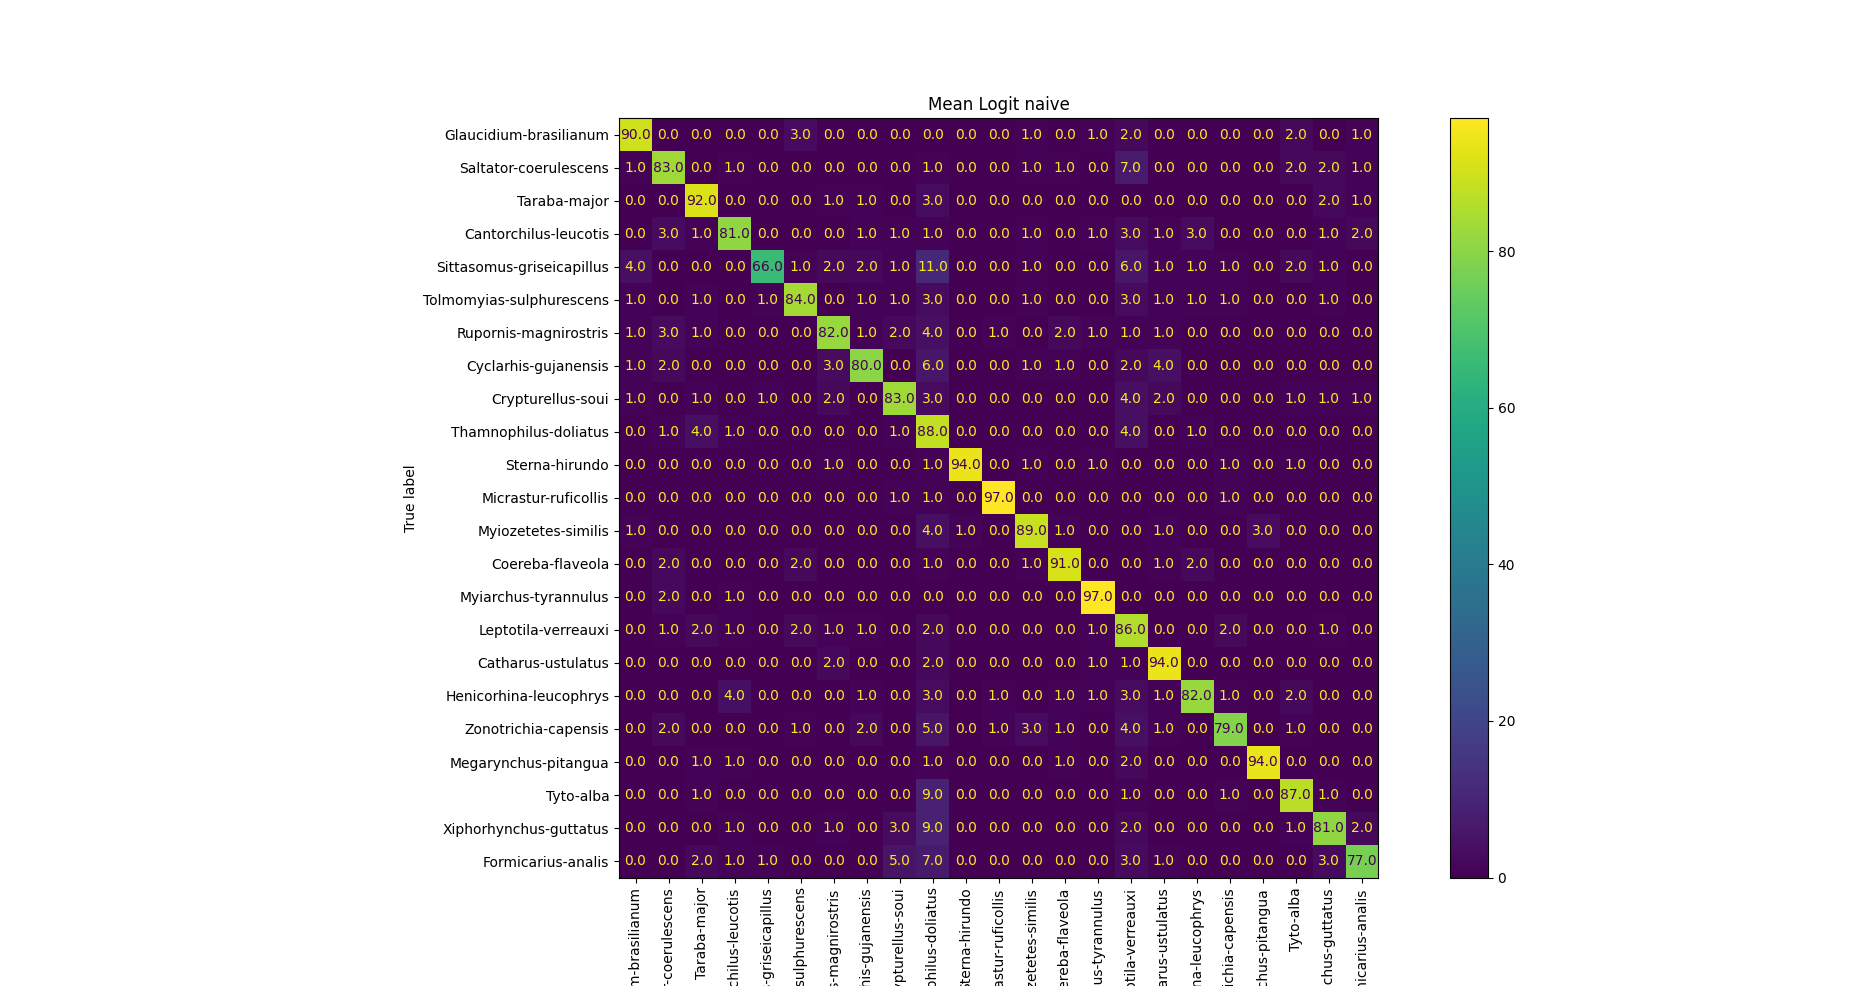
\includegraphics[height=0.7\textheight,width=0.7\textwidth,keepaspectratio]{images/conf_mat_naive.png}
            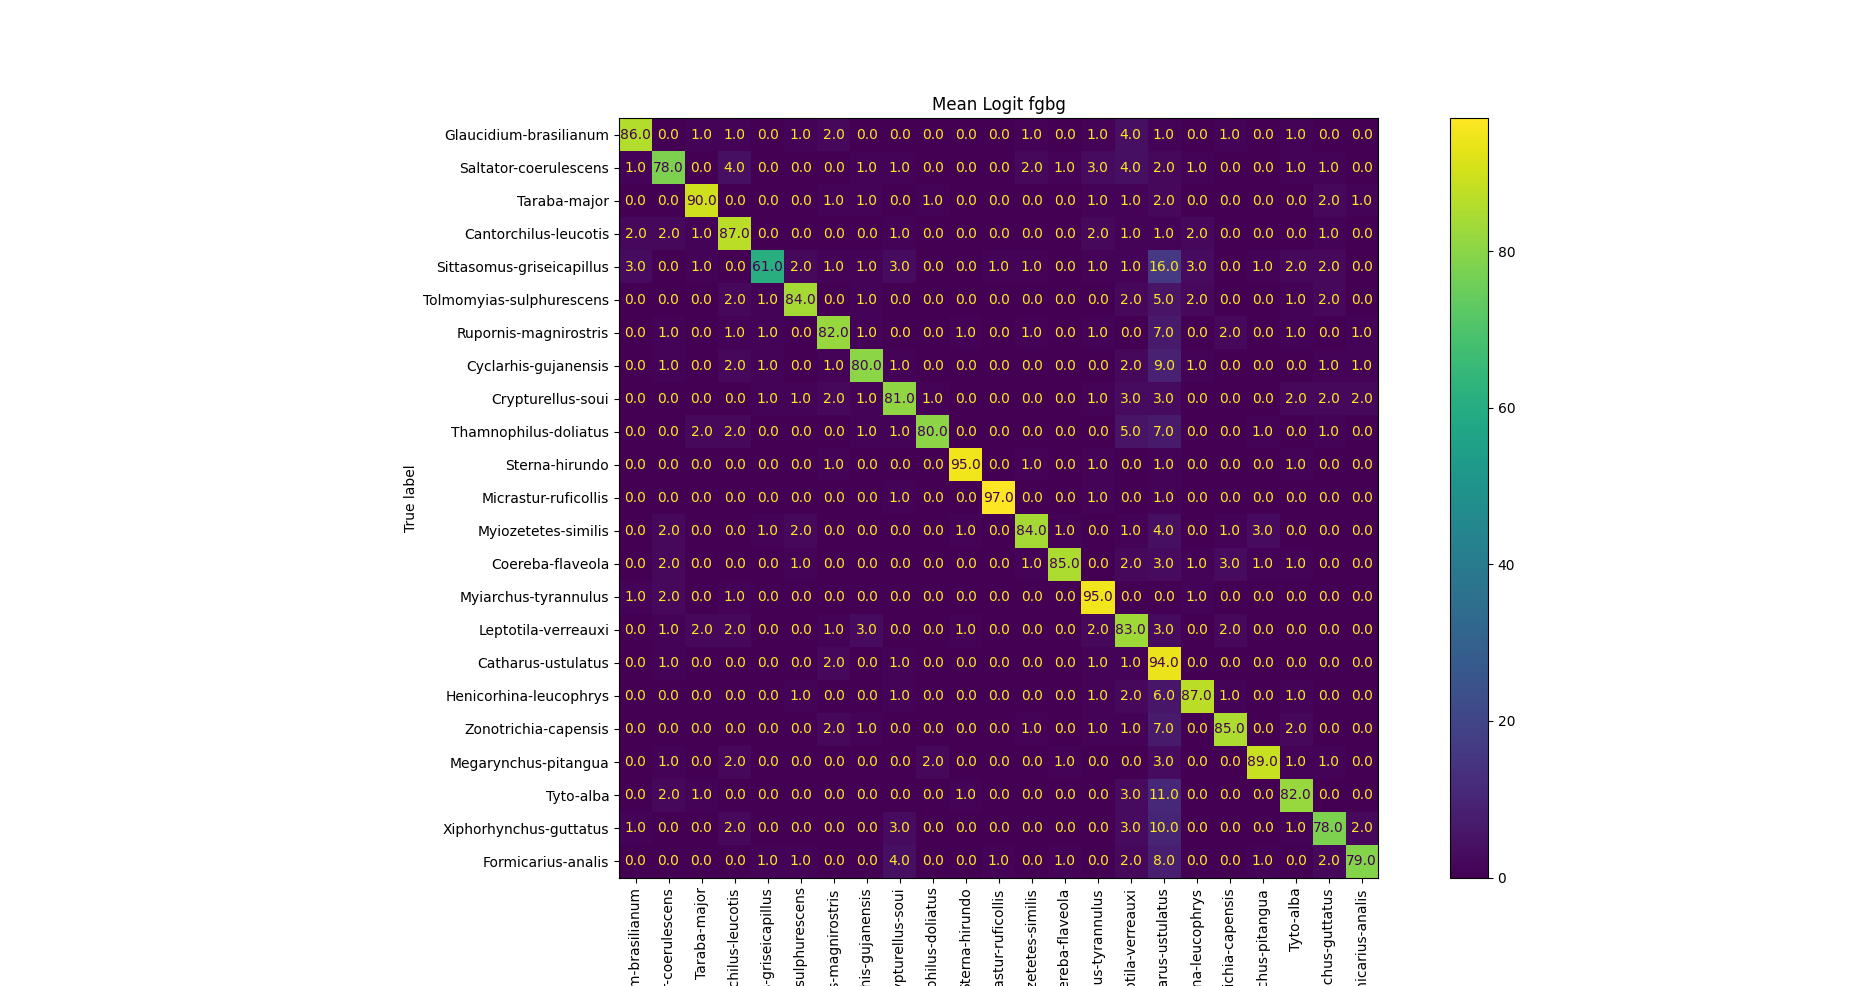
\includegraphics[height=0.7\textheight,width=0.7\textwidth,keepaspectratio]{images/conf_mat_fgbg.png}
        \end{column}
        \begin{column}{0.6\textwidth}
            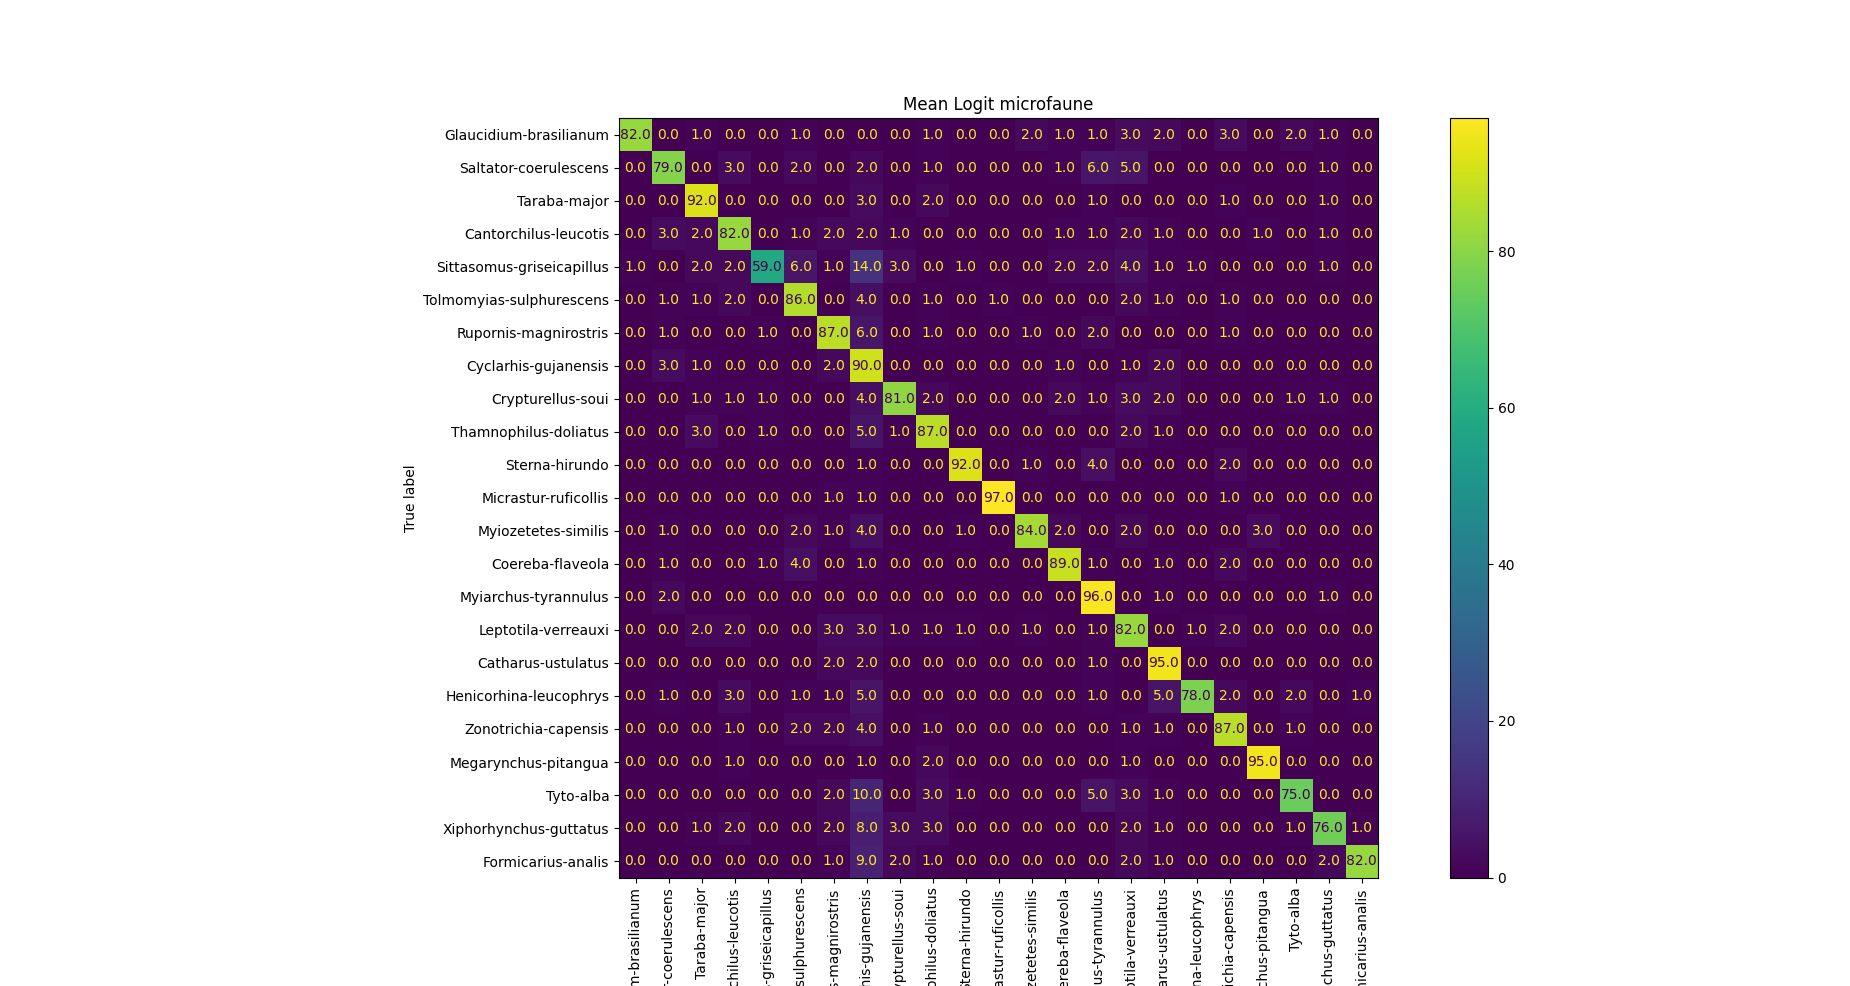
\includegraphics[height=0.7\textheight,width=0.7\textwidth,keepaspectratio]{images/conf_mat_microfaune.png}
            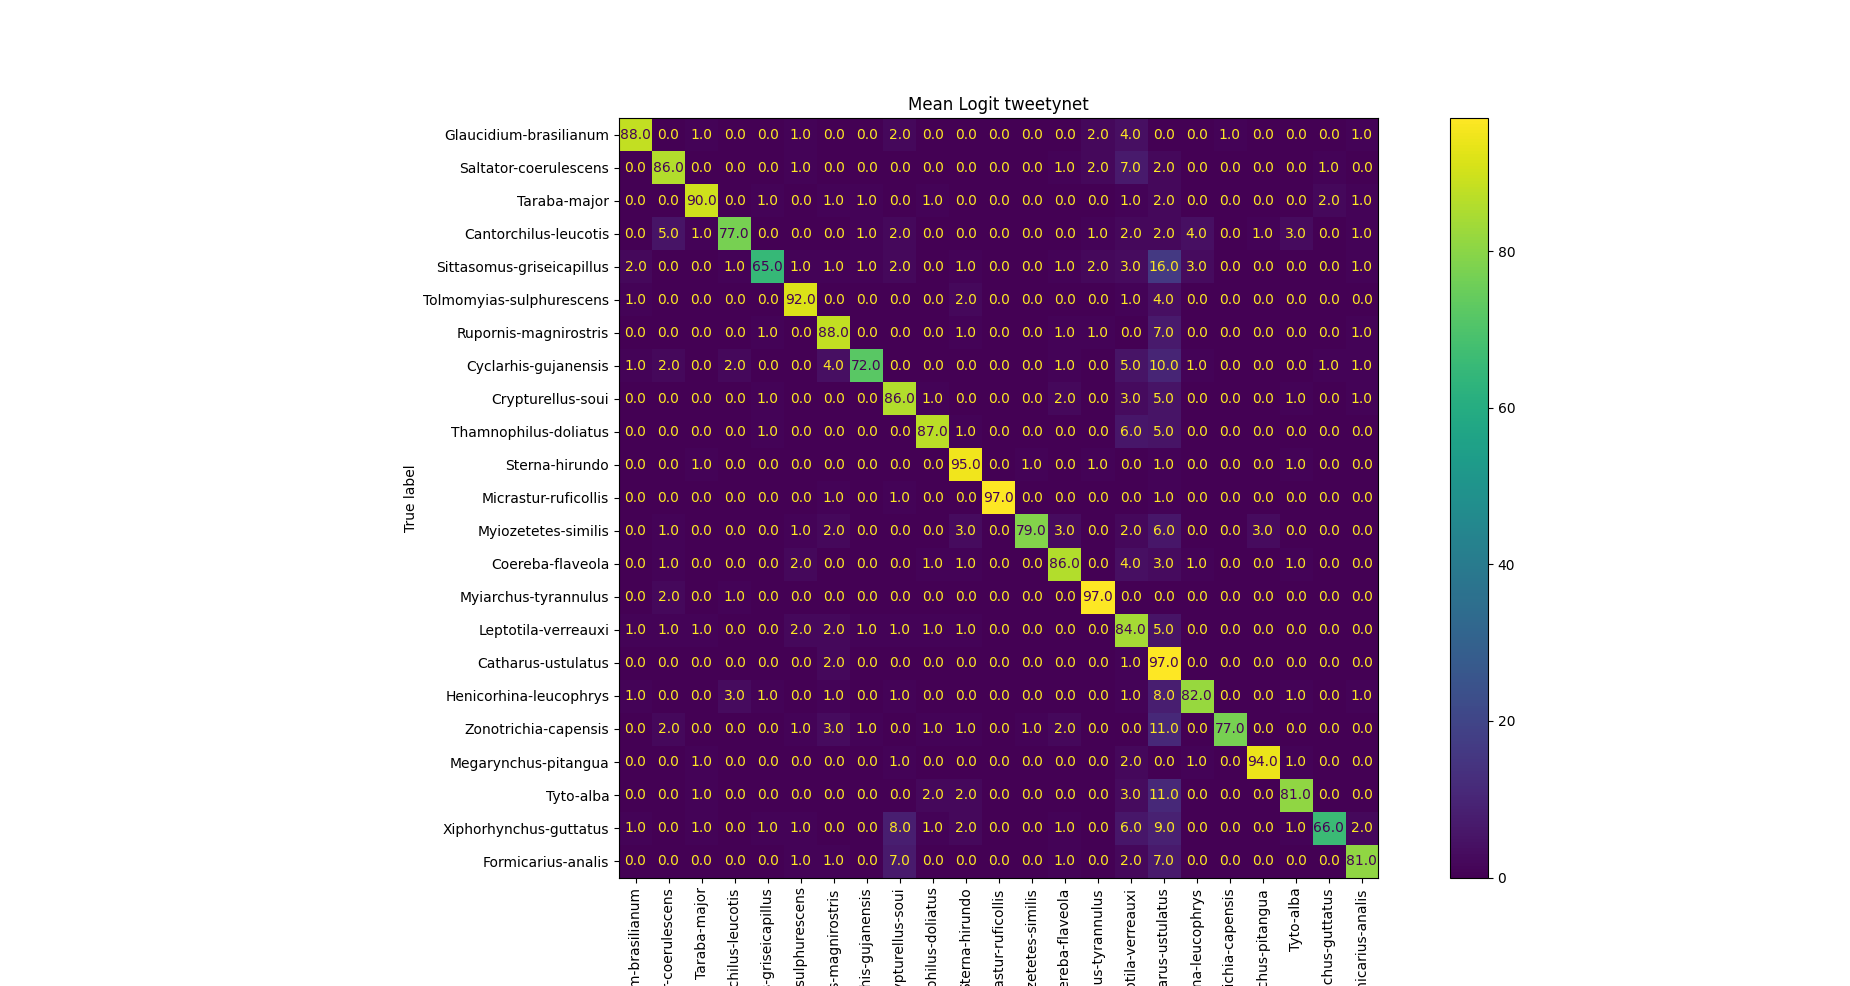
\includegraphics[height=0.7\textheight,width=0.7\textwidth,keepaspectratio]{images/conf_mat_tweetynet.png}
        \end{column}
    \end{columns}
\end{frame}

\begin{frame}{Deep Learning Template Matching Verification}
    \centering
    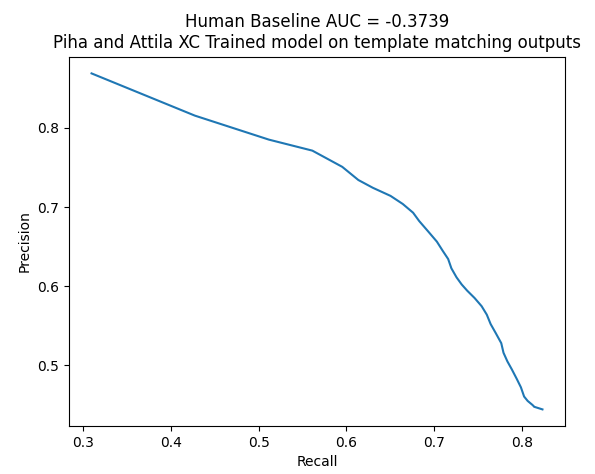
\includegraphics[height=0.7\textheight,width=0.7\textwidth,keepaspectratio]{images/TMV-precision-recall.png}
    \begin{itemize}
        \item 70\% CMAP
        \item songs, not chirps
    \end{itemize}
\end{frame}